% !TEX root = top.tex
% above command is so that compilation is always from top.tex
\section{Background} \label{sec:background}

In this section we describe the platforms HyperFork is built upon, including an
overview of the KVM hypervisor and kvmtool virtual machine monitor.

\subsection{KVM Overview}

KVM is a module within the Linux kernel which provides virtualization support
for running guest machines within Linux processes. A full VMM implementation
will leverage functionality from the KVM module within the kernel through
management layers in userspace. Figure~\ref{fig:kvm-arch} depicts such a
system. The KVM kernel module tracks and maintains most of the sensitive
virtual machine state. Each guest is isolated within a standard Linux process,
which encapsulates both VMM management components and the running guest. The
VMM communicates with the KVM kernel module via a set of ioctls performed on
file descriptors created through the KVM API. Outside of the guest processes,
VMMs often contain CLI or http-based management programs for administrators to
manage VMs. For our implementation, the userspace VMM components are
implemented by kvmtool. These components are conserved across a wide variety of
KVM VMM implementations including Firecracker~\cite{firecracker}.

\begin{figure*}[t]
  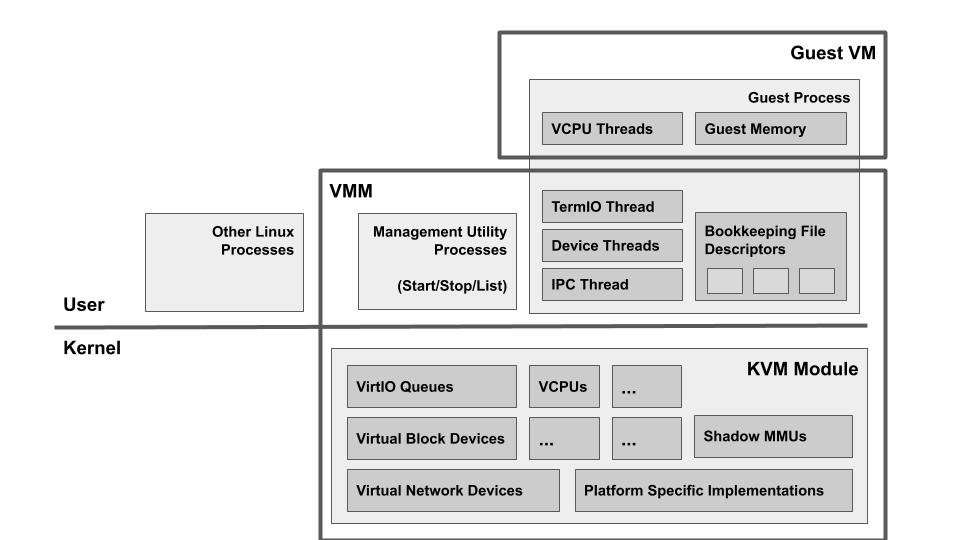
\includegraphics[width=0.8\textwidth]{{figures/kvm-arch}}
  \caption{KVM Software Architecture}
  \label{fig:kvm-arch}
\end{figure*}

\subsection{kvmtool}

kvmtool~\cite{kvmtool} is a VMM implementation for KVM with the minimal
functionality required to boot a fully functional Linux kernel with very basic
virtualized devices. Supported devices include block, network, filesystem,
balloon, hardware random number generation, and console virtual devices, along
with a legacy 8250 serial device. kvmtool is provided as an alternative to
heavier VMM solutions such as QEMU~\cite{qemu}, which supports a wide range of
legacy devices and guest configurations.

We selected kvmtool as our userspace VMM as it offers a very similar set of
functionality to Firecracker, the VMM used to power Amazon Lambda. Both VMMs
are minimal KVM-based implementations which make serverless sandboxes easy to
deploy on Linux environments. By using simple and minimalistic implementations,
startup times and memory footprints are minimized. For increased security in
the cloud, Firecracker uses strict containerization schemes on top of
virtualization-based sandboxing and is implemented in Rust. Firecracker offers
a RESTful API for VM creation and management, and provides no other ways to
communicate with a guest VM. In contrast, kvmtool uses simple IPCs to
communicate and manage guest VMs.

We chose kvmtool over Firecracker because we found that Firecracker was more
difficult to work with due to its Rust codebase and containerization schemes.
kvmtool provides a minimal platform on which to test HyperFork applied to Linux
guests and closely approximates the VMM of an industrial serverless platform.

To virtualize efficiently, kvmtool makes use of a number of threads for
managing vCPUs and emulated devices. Userspace bookkeeping data structures hold
file descriptors which point to the internal VM state maintained by the KVM
kernel module. When the virtual machine is started, kvmtool creates a thread
for each class of device, including the terminal, 8250 serial console, block
devices, and other virtio devices. It then creates several worker threads to
handle arbitrary jobs that may arise from the virtio devices. These tasks
include processing work items from virtio queues and updating the console. In
its default configuration, kvmtool allocates one worker thread for each CPU on
the host machine. As we are virtualizing machines that are much smaller than
the host machine, we limited kvmtool to one worker thread per VM. In addition
to device threads, kvmtool also creates a thread to manage the virtual machines
through IPC calls. This allows administrators to start, pause, stop, and debug
virtual machines using a simple command line interface. Finally, kvmtool
creates one thread per vCPU that proceeds in a loop, invoking the
\texttt{KVM\_RUN} ioctl, then handling any IO requests or interrupts that may
arise. Together, this set of threads enables efficient virtualization of the
guest and its devices.
